\section{Simulation Regler}

\subsection{Simulationsmodell}

\subsubsection{Simulink}
\begin{figure}[h!]
	\centering
	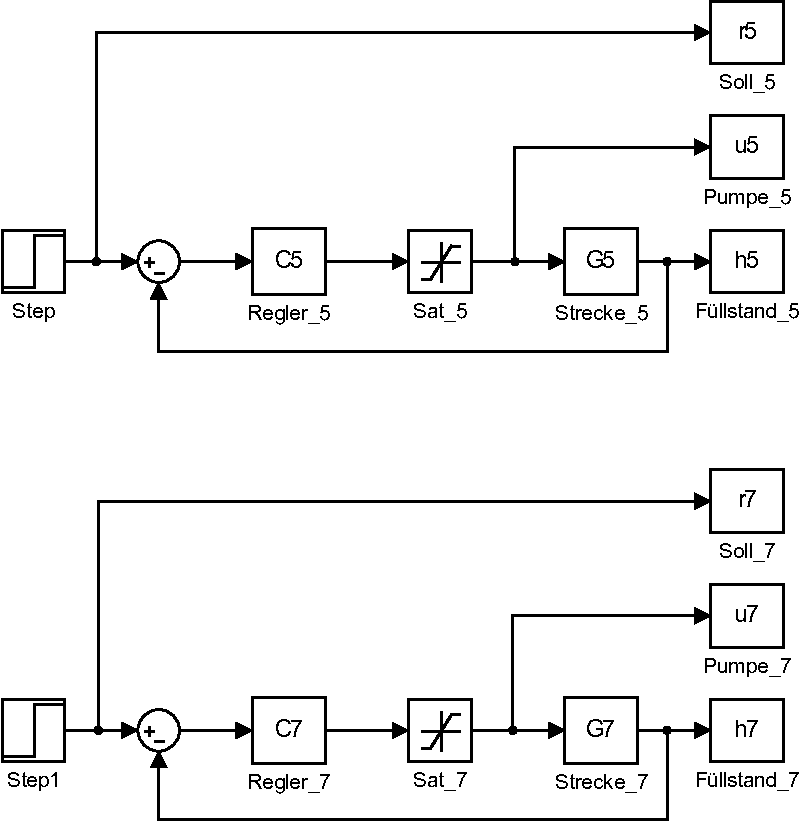
\includegraphics[scale=0.8]{11/model.pdf}
\end{figure}

\subsubsection{MATLAB}
\lstinputlisting{11/regler_siso.m}
% \lstinputlisting{11/plots.m}

\subsection{Simulationsergebnisse}
Die Simulationen ergeben, dass der Regler je nach Arbeitspunkt verschiedene
Ergebnisse liefert. Für einen Sprung um $0.5\si{\centi\meter}$ im optimalen
Arbeitsbereich von $G_5(s)$ erfüllt der modellierte Regler die
Systemanforderungen knapp. Bei einem gleichen Sprung im Arbeitsbereich
von $G_7(s)$ ist ein Schwingen vorhanden welches den Füllstand nicht
an einen stabilen Endwert führt.

\begin{table}[h!]
	\centering
	\begin{tabular}{l c c c c}
		Eigenschaft
			& Spezifikation
			& bei $G_5(s)$
			& bei $G_7(s)$
			& Einheit \\
		\hline
		Genauigkeit
			& 100
			& 100
			& 98 
			& \% \\
		Anregelzeit (0-99\%)
			& $4$
			& 4.2
			& 3.9
			& $\si{\second}$ \\
		Überschwingen
			& $10$
			& 0.6
			& 0
			& \% \\
		Einschwingzeit
			& $5$
			& n.a. 
			& n.a.
			& $\si{\second}$ \\
	\end{tabular}
\end{table}

\begin{figure}[h!]
	\centering
	\begin{subfigure}{0.475\textwidth}
		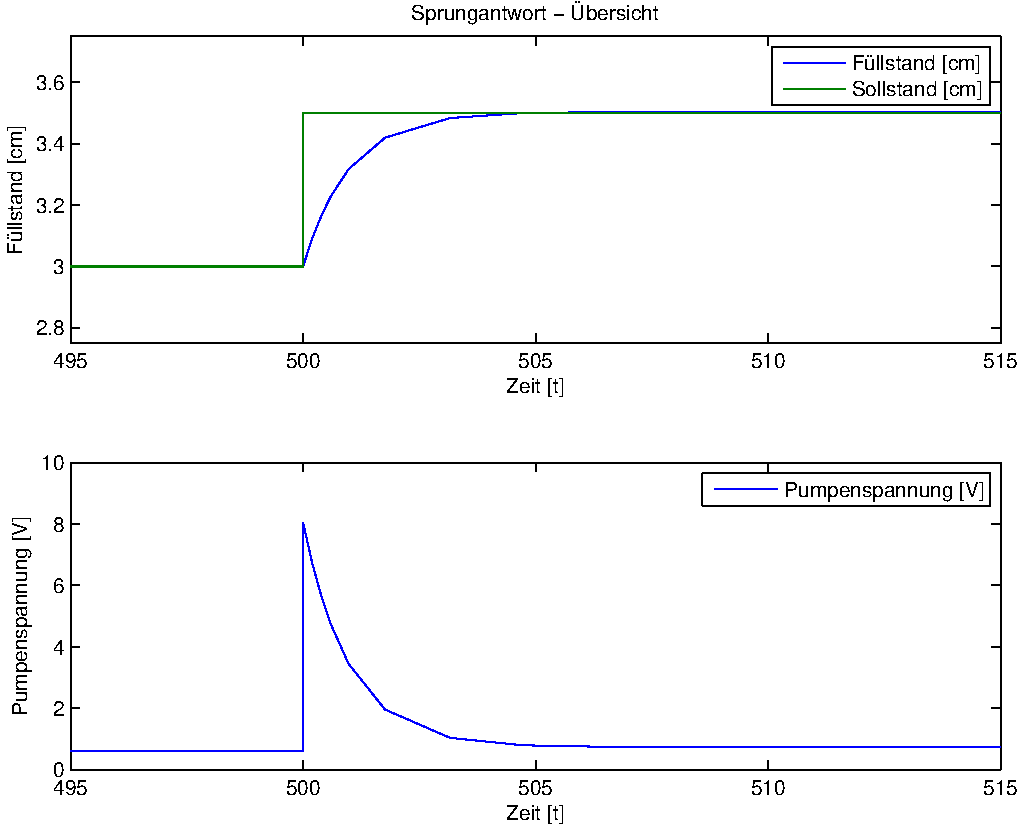
\includegraphics[width=1\textwidth]{11/L5_step_overview_plot.pdf}
		\caption{Schrittantwort im Arbeitsbereich von $G_5(s)$}
	\end{subfigure}
	\hfill{}
	\begin{subfigure}{0.475\textwidth}
		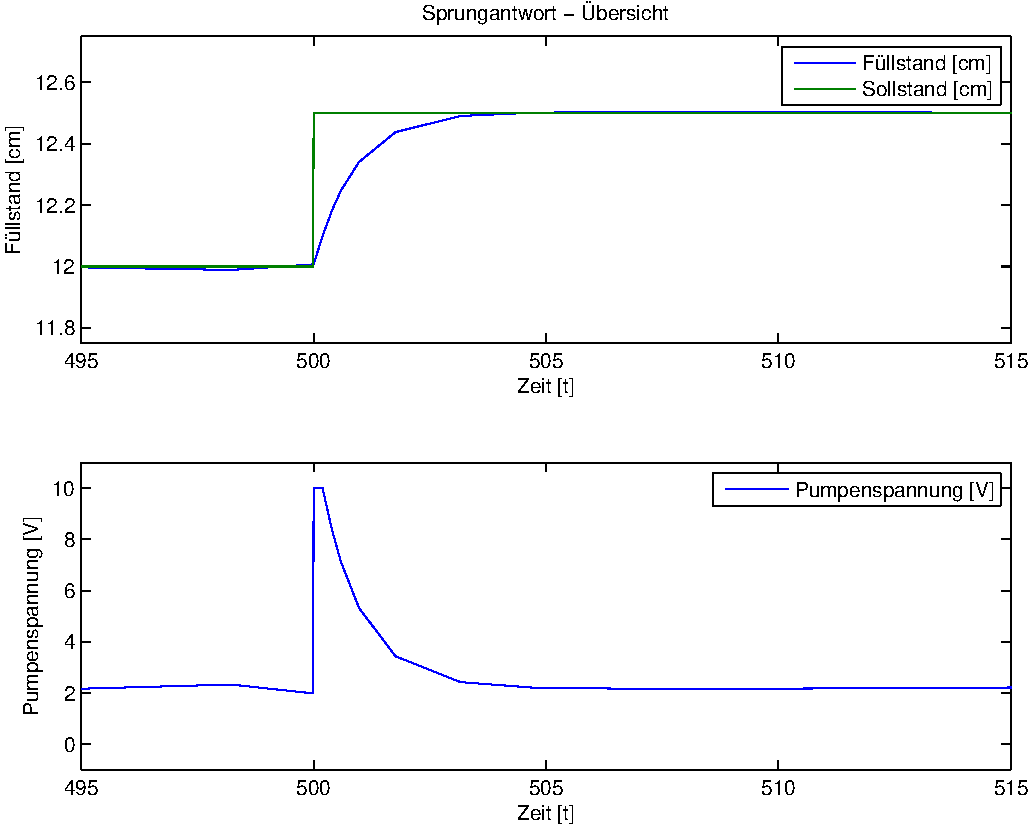
\includegraphics[width=1\textwidth]{11/L7_step_overview_plot.pdf}
		\caption{Schrittantwort im Arbeitsbereich von $G_7(s)$}
	\end{subfigure}
	\caption{Übersicht der Schrittantworten mit dem SISO-Tool optimierten Regler}
\end{figure}

\begin{figure}[h!]
	\begin{subfigure}{0.475\textwidth}
		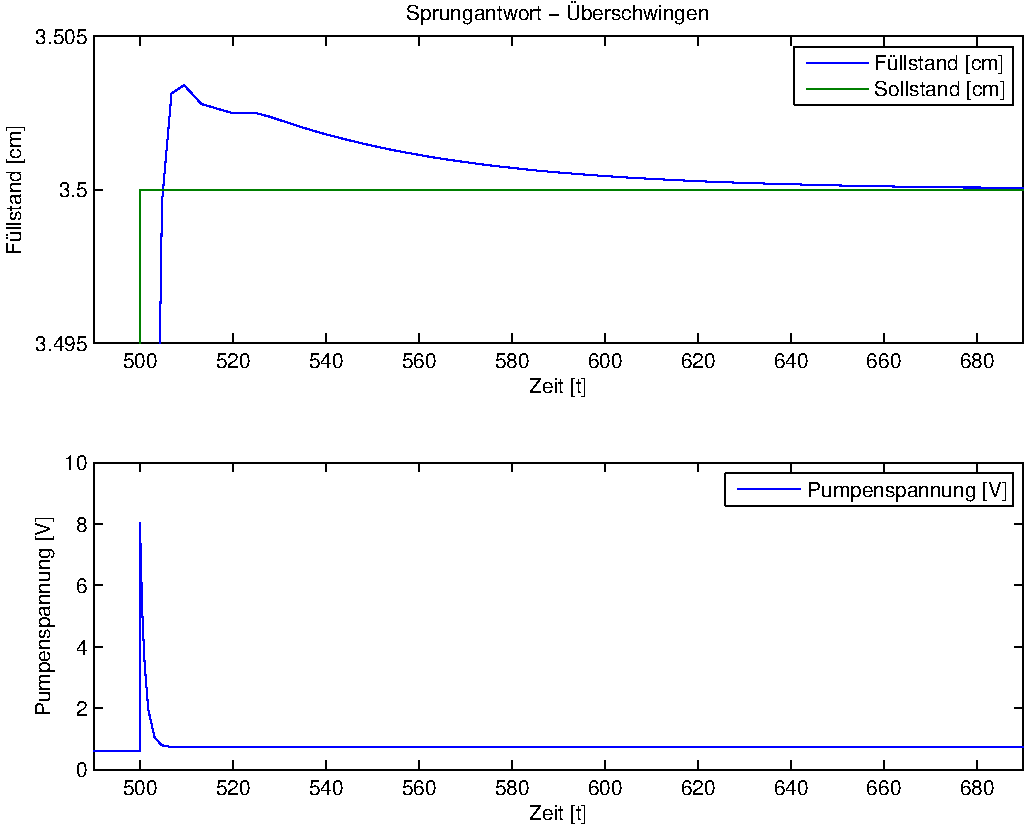
\includegraphics[width=1\textwidth]{11/L5_step_overshoot_plot.pdf}
		\caption{Überschwingen im Arbeitsbereich von $G_5(s)$}
	\end{subfigure}
	\hfill{}
	\begin{subfigure}{0.475\textwidth}
		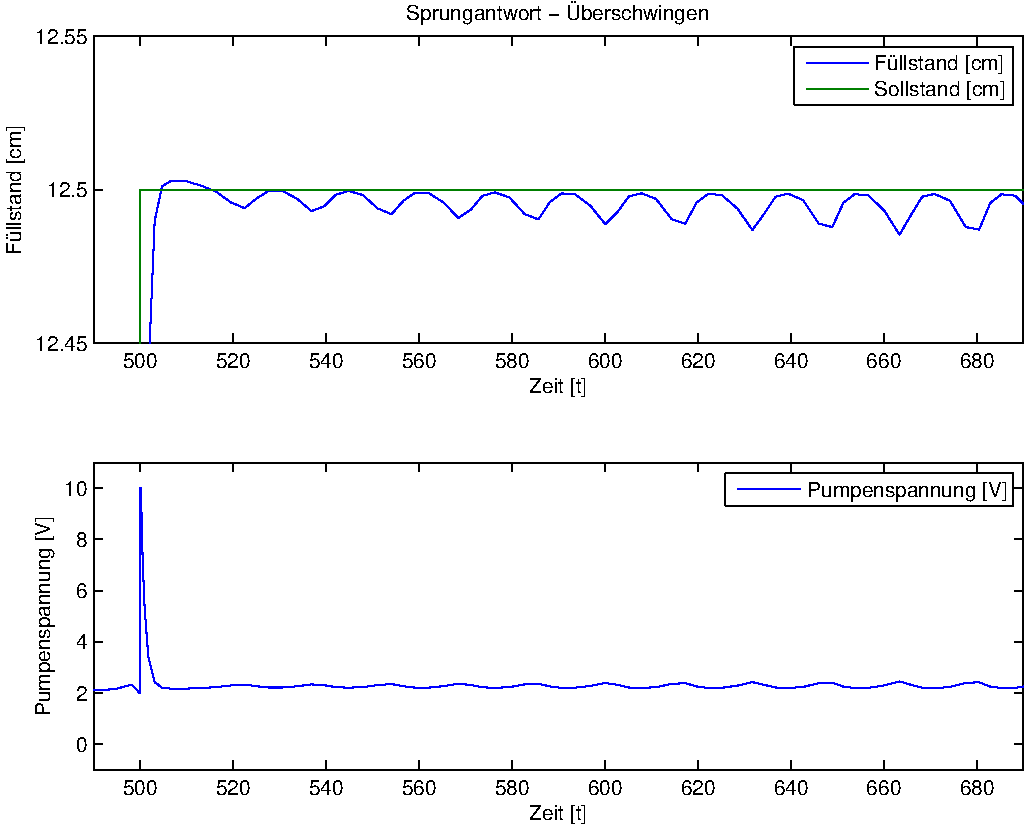
\includegraphics[width=1\textwidth]{11/L7_step_overshoot_plot.pdf}
		\caption{Überschwingen im Arbeitsbereich von $G_7(s)$}
	\end{subfigure}
	\caption{Überschwingen für den mit dem SISO-Tool optimierten Regler}
\end{figure}

